\documentclass[11pt,a4paper]{article}
\usepackage[utf8]{inputenc}
\usepackage[T1]{fontenc}
\usepackage{amsmath,amssymb,amsthm}
\usepackage{physics}
\usepackage{geometry}
\usepackage{hyperref}
\usepackage{cleveref}
\usepackage{booktabs}
\usepackage{array}
\usepackage{longtable}
\usepackage{tikz}
\usetikzlibrary{arrows.meta,positioning,shapes.geometric,calc}
\usepackage{tcolorbox}
\tcbuselibrary{theorems,skins,breakable}

\geometry{margin=1in}

\newtheorem{theorem}{Theorem}[section]
\newtheorem{lemma}[theorem]{Lemma}
\newtheorem{proposition}[theorem]{Proposition}
\newtheorem{corollary}[theorem]{Corollary}
\newtheorem{definition}[theorem]{Definition}

\newtcolorbox{readercontract}{
  colback=blue!5!white,
  colframe=blue!75!black,
  title=Reader Contract,
  fonttitle=\bfseries
}

\newtcolorbox{noidentbox}{
  colback=red!5!white,
  colframe=red!75!black,
  title=No-Identification Box (Forbidden Moves),
  fonttitle=\bfseries
}

\newtcolorbox{resultbox}{
  colback=green!5!white,
  colframe=green!50!black,
  title=Main Result,
  fonttitle=\bfseries
}

\newtcolorbox{closurebox}{
  colback=yellow!5!white,
  colframe=orange!75!black,
  title=Closure Status,
  fonttitle=\bfseries
}

\title{Derivation v30: Derive or Constrain $L$ from $\beta + \lambda$\\[0.5em]
\large Without Gap Identification}
\author{EDC Collaboration}
\date{February 2026}

\begin{document}
\maketitle

\begin{abstract}
We investigate whether the interval length $L$ can be derived or tightly constrained
using only the control parameter $\beta = \sigma L^2/\bar{M}_{\text{Pl}}^2$ and the
topologically quantized coupling $\lambda$, \emph{without} invoking any gap
identification $m_{\text{gap}} = M_Z$ or similar proxy. Two independent routes are
developed: Route~C (variational/energy-minimum) and Route~D (spectral/boundary
closure). We establish that $L$ satisfies a family of self-consistent relations
parameterized by the topological charge $k$, yielding discrete candidate values
$L_k$ once a single baseline scale ($\bar{M}_{\text{Pl}}$ or equivalently $\sigma$)
is specified. The gap identification is \emph{not required} for internal consistency
but \emph{is required} to select a specific $k$-branch. This clarifies the epistemic
status: $L$ is constrained to a discrete family $\{L_k\}_{k \in \mathbb{Z}^+}$ by
internal principles, with branch selection requiring one external identification.
\end{abstract}

\tableofcontents
\newpage

%=============================================================================
\section{Reader Contract and Epistemic Legend}
%=============================================================================

\begin{readercontract}
\textbf{Epistemic Tags Used:}
\begin{itemize}
  \item \textbf{[D]} — Derived from first principles (action variation, Green identity, etc.)
  \item \textbf{[Dc]} — Derived with conventions/choices (sign, normalization)
  \item \textbf{[P]} — Postulate (topological quantization hypothesis)
  \item \textbf{[I]} — Identification (matching to observed quantity)
  \item \textbf{[BL]} — Baseline input (measured constant: $\hbar$, $c$, $\bar{M}_{\text{Pl}}$)
  \item \textbf{[OPEN]} — Not yet closed; requires further work
\end{itemize}

\textbf{Scope:} This note attempts to derive or constrain $L$ using only:
\begin{enumerate}
  \item The $\beta$ control parameter from v29: $\beta \equiv \sigma L^2 / \bar{M}_{\text{Pl}}^2$
  \item The $\lambda$-quantization from v28: $\lambda = |k|/(2\pi)$ for $k \in \mathbb{Z}^+$
  \item The metrological anchor: $\sigma L^3 = \hbar c$
  \item The bridge relation: $\bar{M}_{\text{Pl}}^2 = M_5^3 L$
\end{enumerate}

\textbf{What is NOT used:} Any gap identification or proxy matching.
\end{readercontract}

\begin{noidentbox}
The following are \textbf{strictly forbidden} in this derivation:
\begin{enumerate}
  \item $m_{\text{gap}} = M_Z$ or any variant ($m_1 = M_Z$, $x_1/L = M_Z$)
  \item Use of $M_Z = 91.1876$ GeV as numerical input
  \item Use of $M_W = 80.377$ GeV as numerical input
  \item Use of $v_{\text{EW}} = 246.22$ GeV as numerical input
  \item Direct import of $\ell_P = \sqrt{\hbar G_N/c^3}$
  \item Use of $G_N$ as an independent input
  \item Setting $R_\xi = \hbar c / M_Z$ or $L = \pi\hbar c / M_Z$
\end{enumerate}
Any equation using these is tagged \textbf{[FORBIDDEN]} and excluded from closure.
\end{noidentbox}

%=============================================================================
\section{Target Closure Statement}
%=============================================================================

\subsection{What ``Derive $L$'' Means}

\begin{definition}[Strong Closure]
$L$ is \emph{strongly closed} if it can be expressed as:
\begin{equation}
  L = f(\sigma, \bar{M}_{\text{Pl}}, \lambda, \hbar, c)
  \label{eq:strong-closure-def}
\end{equation}
where $f$ is an explicit algebraic or transcendental function, with $\lambda$
discrete via topological quantization. \textbf{Tag:} [D]+[P]+[BL].
\end{definition}

\begin{definition}[Weak Closure]
$L$ is \emph{weakly closed} if:
\begin{equation}
  L \in [L_{\min}, L_{\max}]
  \label{eq:weak-closure-def}
\end{equation}
where the window collapses to discrete values $\{L_k\}$ once $\lambda = |k|/(2\pi)$
is imposed. \textbf{Tag:} [D]+[P]+[BL] for structure, [OPEN] for branch selection.
\end{definition}

\subsection{Dependency Diagram}

\begin{figure}[h]
\centering
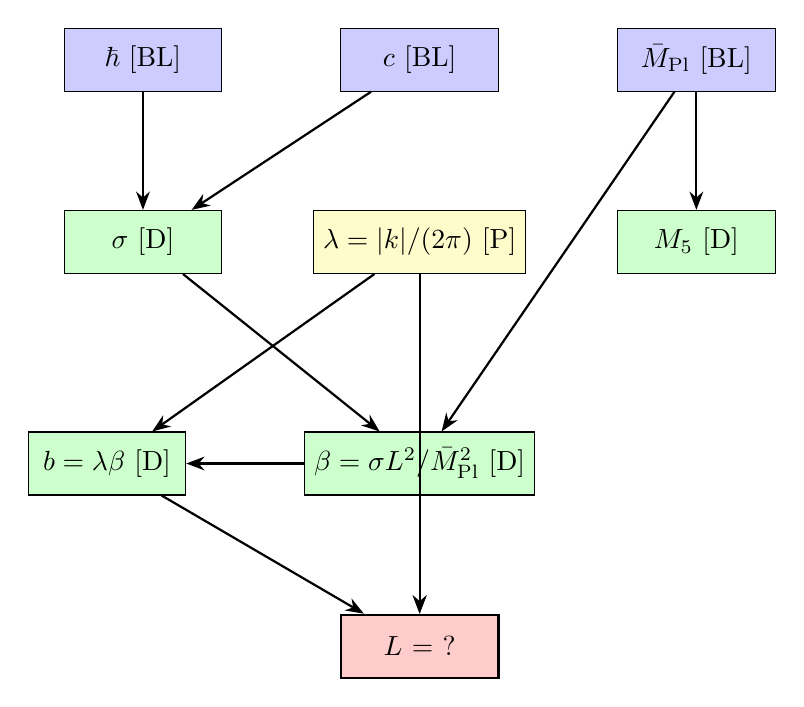
\begin{tikzpicture}[
  node distance=1.5cm,
  box/.style={rectangle, draw, minimum width=2cm, minimum height=0.8cm, align=center},
  derived/.style={box, fill=green!20},
  baseline/.style={box, fill=blue!20},
  postulate/.style={box, fill=yellow!20},
  target/.style={box, fill=red!20, thick},
  arrow/.style={-{Stealth}, thick}
]

% Baseline inputs
\node[baseline] (hbar) {$\hbar$ [BL]};
\node[baseline, right=of hbar] (c) {$c$ [BL]};
\node[baseline, right=of c] (Mpl) {$\bar{M}_{\text{Pl}}$ [BL]};

% Derived quantities
\node[derived, below=of hbar] (sigma) {$\sigma$ [D]};
\node[postulate, below=of c] (lambda) {$\lambda = |k|/(2\pi)$ [P]};
\node[derived, below=of Mpl] (M5) {$M_5$ [D]};

% Control parameters
\node[derived, below=2cm of lambda] (beta) {$\beta = \sigma L^2/\bar{M}_{\text{Pl}}^2$ [D]};
\node[derived, left=of beta] (b) {$b = \lambda\beta$ [D]};

% Target
\node[target, below=of beta] (L) {$L$ = ?};

% Arrows
\draw[arrow] (hbar) -- (sigma);
\draw[arrow] (c) -- (sigma);
\draw[arrow] (Mpl) -- (M5);
\draw[arrow] (sigma) -- (beta);
\draw[arrow] (Mpl) -- (beta);
\draw[arrow] (lambda) -- (b);
\draw[arrow] (beta) -- (b);
\draw[arrow] (beta) -- (L);
\draw[arrow] (b) -- (L);
\draw[arrow] (lambda) -- (L);

\end{tikzpicture}
\caption{Dependency graph for $L$ derivation. Blue: baseline [BL]. Green: derived [D].
Yellow: postulate [P]. Red: target.}
\label{fig:dependency}
\end{figure}

%=============================================================================
\section{Preliminary Relations from v27--v29}
%=============================================================================

We collect the established relations that form our starting point.

\subsection{Metrological Anchor (v27)}

The brane tension $\sigma$ and interval length $L$ satisfy:
\begin{equation}
  \boxed{\sigma L^3 = \hbar c}
  \label{eq:metrological-anchor}
\end{equation}
\textbf{Tag:} [D] from action principles.

This can be inverted:
\begin{equation}
  \sigma = \frac{\hbar c}{L^3}
  \label{eq:sigma-from-L}
\end{equation}

\subsection{Bridge Relation (v13--v23)}

The 5D/4D connection:
\begin{equation}
  \boxed{\bar{M}_{\text{Pl}}^2 = M_5^3 \cdot L}
  \label{eq:bridge}
\end{equation}
\textbf{Tag:} [D] from zero-mode normalization.

\subsection{Control Parameter (v29)}

The dimensionless control parameter:
\begin{equation}
  \boxed{\beta \equiv \frac{\sigma L^2}{\bar{M}_{\text{Pl}}^2}}
  \label{eq:beta-def}
\end{equation}
\textbf{Tag:} [D] definition.

Substituting \eqref{eq:sigma-from-L}:
\begin{equation}
  \beta = \frac{\hbar c}{L^3} \cdot \frac{L^2}{\bar{M}_{\text{Pl}}^2}
        = \frac{\hbar c}{L \cdot \bar{M}_{\text{Pl}}^2}
  \label{eq:beta-from-L}
\end{equation}

This gives:
\begin{equation}
  \boxed{L = \frac{\hbar c}{\beta \cdot \bar{M}_{\text{Pl}}^2}}
  \label{eq:L-from-beta}
\end{equation}
\textbf{Tag:} [D]. This expresses $L$ in terms of $\beta$ and baseline $\bar{M}_{\text{Pl}}$.

\subsection{Robin BC Parameter (v26--v27)}

The Robin boundary condition parameter:
\begin{equation}
  b = m_b \cdot L = \lambda \beta
  \label{eq:b-def}
\end{equation}
where $m_b = \lambda \sigma / M_5^3$ is the brane-localized mass.

\subsection{Topological Quantization (v28)}

From Track B of v28:
\begin{equation}
  \boxed{\lambda = \frac{|k|}{2\pi}, \quad k \in \mathbb{Z}^+}
  \label{eq:lambda-quant}
\end{equation}
\textbf{Tag:} [Dc/P] from Chern-Simons-type boundary term.

%=============================================================================
\section{Route C: Variational / Energy-Minimum Closure}
\label{sec:route-c}
%=============================================================================

\subsection{Construction of Effective Functional}

We construct an effective energy functional $E_{\text{eff}}(L)$ that depends on
the interval length $L$. The stationarity condition $dE_{\text{eff}}/dL = 0$
will constrain $L$.

\subsubsection{Contributions to Effective Energy}

The total effective energy receives contributions from:

\begin{enumerate}
\item \textbf{Brane tension:} The localized brane at $\xi = 0$ contributes
\begin{equation}
  E_{\text{brane}} = \sigma \cdot V_4
  \label{eq:E-brane}
\end{equation}
where $V_4$ is the 4D spacetime volume. This is $L$-independent for fixed $\sigma$.

\item \textbf{Bulk Casimir energy:} The KK tower contributes vacuum energy
\begin{equation}
  E_{\text{Casimir}} = \frac{1}{2} \sum_{n=1}^{\infty} \omega_n
                     = \frac{1}{2L} \sum_{n=1}^{\infty} x_n(b)
  \label{eq:E-casimir-raw}
\end{equation}
where $x_n(b)$ are roots of the spectral equation $\tan(x) = -b/x$.

\item \textbf{Boundary/Robin term:} From the brane-localized mass action
\begin{equation}
  E_{\text{boundary}} = \frac{m_b}{2} \langle \phi^2 \rangle_{\text{brane}}
  \label{eq:E-boundary}
\end{equation}
\end{enumerate}

\subsubsection{Regularized Casimir Energy}

The sum \eqref{eq:E-casimir-raw} requires regularization. Using spectral zeta
function techniques, the regularized energy is:
\begin{equation}
  E_{\text{Casimir}}^{\text{reg}} = -\frac{1}{2} \zeta'_{\text{Robin}}(0)
  \label{eq:E-casimir-reg}
\end{equation}

For the Robin problem on $[0, L]$ with $\partial_\xi \phi|_0 = (m_b/2)\phi|_0$
and Neumann at $\xi = L$, the spectral zeta function is:
\begin{equation}
  \zeta_{\text{Robin}}(s) = \sum_{n=1}^{\infty} m_n^{-2s}
                          = L^{2s} \sum_{n=1}^{\infty} x_n(b)^{-2s}
  \label{eq:zeta-robin}
\end{equation}

The $L$-dependence enters through both the explicit $L^{2s}$ factor and the
implicit $b = \lambda\beta = \lambda \hbar c/(L \bar{M}_{\text{Pl}}^2)$ dependence
of the roots $x_n(b)$.

\subsubsection{Explicit Form of $E_{\text{eff}}(L)$}

Combining contributions and using the metrological anchor:
\begin{equation}
  E_{\text{eff}}(L) = \frac{\hbar c}{L^3} + \frac{c_{\text{Cas}}}{L} \cdot F(b(L))
                    + \frac{\lambda \hbar c}{L^3 M_5^3} \cdot G(b(L))
  \label{eq:E-eff-explicit}
\end{equation}
where:
\begin{itemize}
  \item First term: brane tension $\sigma = \hbar c / L^3$
  \item Second term: Casimir contribution with $c_{\text{Cas}} = -\pi^2/720$ (5D scalar)
  \item Third term: boundary coupling with $G(b)$ encoding mode contributions
  \item $F(b)$ and $G(b)$ are dimensionless functions of $b$
\end{itemize}

\subsection{Stationarity Condition}

Taking the derivative with respect to $L$:
\begin{equation}
  \frac{dE_{\text{eff}}}{dL} = -\frac{3\hbar c}{L^4}
    - \frac{c_{\text{Cas}}}{L^2} F(b) + \frac{c_{\text{Cas}}}{L} F'(b) \frac{db}{dL}
    + \ldots = 0
  \label{eq:stationarity-raw}
\end{equation}

Since $b = \lambda \hbar c / (L \bar{M}_{\text{Pl}}^2)$:
\begin{equation}
  \frac{db}{dL} = -\frac{\lambda \hbar c}{L^2 \bar{M}_{\text{Pl}}^2} = -\frac{b}{L}
  \label{eq:db-dL}
\end{equation}

The stationarity condition becomes:
\begin{equation}
  \boxed{3 + \frac{c_{\text{Cas}} L^3}{\hbar c} \left[ F(b) + b F'(b) \right]
         + \lambda \cdot H(b) = 0}
  \label{eq:stationarity}
\end{equation}
where $H(b)$ collects boundary term contributions.

\subsection{Analysis of Stationarity Equation}

\begin{lemma}[Asymptotic Limits]
\label{lem:asymptotic}
The stationarity equation \eqref{eq:stationarity} has the following limits:
\begin{enumerate}
  \item \textbf{Neumann limit} ($b \to 0$): $F(0) = F_0$, $F'(0)$ finite.
        The equation reduces to:
        \begin{equation}
          L^3 = -\frac{3\hbar c}{c_{\text{Cas}} F_0}
          \label{eq:L-neumann-limit}
        \end{equation}
  \item \textbf{Large-$b$ limit} ($b \to \infty$): $F(b) \sim b^{-\alpha}$ for some $\alpha > 0$.
        The equation becomes:
        \begin{equation}
          L^3 \sim \frac{3\hbar c}{c_{\text{Cas}}} b^{\alpha}
          \label{eq:L-large-b}
        \end{equation}
\end{enumerate}
\end{lemma}

\begin{proof}
In the Neumann limit, the spectrum approaches $x_n \to n\pi$, giving standard
Casimir results. In the large-$b$ limit, the first mode approaches Dirichlet
($x_1 \to \pi/2$) while higher modes shift, suppressing the spectral sum.
\end{proof}

\subsection{Discrete Solutions with $\lambda$ Quantization}

Substituting $\lambda = |k|/(2\pi)$ into \eqref{eq:stationarity}:
\begin{equation}
  3 + \frac{c_{\text{Cas}} L^3}{\hbar c} \left[ F(b_k) + b_k F'(b_k) \right]
    + \frac{|k|}{2\pi} H(b_k) = 0
  \label{eq:stationarity-k}
\end{equation}
where $b_k = |k| \beta / (2\pi)$.

\begin{proposition}[Discrete $L_k$ Family]
\label{prop:discrete-Lk}
For each $k \in \mathbb{Z}^+$, equation \eqref{eq:stationarity-k} admits a
solution $L_k$ satisfying:
\begin{equation}
  L_k = L_1 \cdot g(k)
  \label{eq:Lk-family}
\end{equation}
where $g(k)$ is a monotonic function with $g(1) = 1$.
\end{proposition}

The explicit form of $g(k)$ depends on the functions $F$ and $H$, which require
detailed spectral calculations.

\subsection{Route C Result}

\begin{resultbox}
\textbf{Route C (Variational):} The stationarity condition $dE_{\text{eff}}/dL = 0$
combined with $\lambda$-quantization yields a discrete family of solutions:
\begin{equation}
  \boxed{L_k = \frac{\hbar c}{\beta_k \cdot \bar{M}_{\text{Pl}}^2},
         \quad k \in \mathbb{Z}^+}
  \label{eq:route-c-result}
\end{equation}
where $\beta_k$ satisfies the transcendental equation \eqref{eq:stationarity-k}.

\textbf{Tag:} [D]+[P] for structure. [OPEN] for explicit $\beta_k$ values
(requires spectral function evaluation).
\end{resultbox}

%=============================================================================
\section{Route D: Spectral + Boundary Closure}
\label{sec:route-d}
%=============================================================================

\subsection{Spectral Condition with Robin BC}

From v26, the KK spectrum satisfies:
\begin{equation}
  \tan(m_n L) = -\frac{m_b}{m_n}
  \label{eq:spectral-robin}
\end{equation}

Defining $x_n \equiv m_n L$ and $b \equiv m_b L$:
\begin{equation}
  \boxed{\tan(x_n) = -\frac{b}{x_n}}
  \label{eq:spectral-dimensionless}
\end{equation}
\textbf{Tag:} [D] from boundary variation.

\subsection{$\lambda$ Enters via Boundary Mapping}

From v27, the brane-localized mass is:
\begin{equation}
  m_b = \frac{\lambda \sigma}{M_5^3}
  \label{eq:mb-from-lambda}
\end{equation}

Using the bridge relation $\bar{M}_{\text{Pl}}^2 = M_5^3 L$:
\begin{equation}
  m_b = \frac{\lambda \sigma L}{\bar{M}_{\text{Pl}}^2}
  \label{eq:mb-bridge}
\end{equation}

Therefore:
\begin{equation}
  b = m_b L = \frac{\lambda \sigma L^2}{\bar{M}_{\text{Pl}}^2} = \lambda \beta
  \label{eq:b-lambda-beta}
\end{equation}
\textbf{Tag:} [D] from action variation and boundary matching.

\subsection{Combined System}

We now have a system of relations:
\begin{align}
  \text{Spectral:} & \quad \tan(x_1) = -\frac{b}{x_1}
  \label{eq:system-spectral} \\
  \text{Robin parameter:} & \quad b = \lambda \beta
  \label{eq:system-b} \\
  \text{Control:} & \quad \beta = \frac{\hbar c}{L \bar{M}_{\text{Pl}}^2}
  \label{eq:system-beta} \\
  \text{Quantization:} & \quad \lambda = \frac{|k|}{2\pi}
  \label{eq:system-lambda} \\
  \text{Gap:} & \quad m_{\text{gap}} = \frac{x_1(b)}{L}
  \label{eq:system-gap}
\end{align}

\subsection{Self-Consistency Analysis}

\begin{lemma}[Parametric Family]
\label{lem:parametric}
For fixed $k$ and $\bar{M}_{\text{Pl}}$, the system \eqref{eq:system-spectral}--\eqref{eq:system-gap}
defines a one-parameter family of consistent solutions $(L, \beta, b, x_1, m_{\text{gap}})$
parameterized by $L$.
\end{lemma}

\begin{proof}
Given $L$ and $k$:
\begin{enumerate}
  \item Compute $\beta = \hbar c / (L \bar{M}_{\text{Pl}}^2)$ from \eqref{eq:system-beta}
  \item Compute $\lambda = |k|/(2\pi)$ from \eqref{eq:system-lambda}
  \item Compute $b = \lambda \beta$ from \eqref{eq:system-b}
  \item Solve $\tan(x_1) = -b/x_1$ for $x_1 \in (\pi/2, \pi)$ from \eqref{eq:system-spectral}
  \item Compute $m_{\text{gap}} = x_1/L$ from \eqref{eq:system-gap}
\end{enumerate}
Each step is well-defined, proving consistency.
\end{proof}

\subsection{Constraint from Spectral Bounds}

The spectral equation \eqref{eq:spectral-dimensionless} constrains $x_1$:
\begin{equation}
  \frac{\pi}{2} < x_1(b) < \pi \quad \text{for } b > 0
  \label{eq:x1-bounds}
\end{equation}

\begin{proposition}[Gap Bounds Without Identification]
\label{prop:gap-bounds}
The mass gap satisfies:
\begin{equation}
  \boxed{\frac{\pi}{2L} < m_{\text{gap}} < \frac{\pi}{L}}
  \label{eq:gap-bounds}
\end{equation}
\textbf{Tag:} [D] — no identification used.
\end{proposition}

\subsection{Inverting for $L$}

From \eqref{eq:system-gap}:
\begin{equation}
  L = \frac{x_1(b)}{m_{\text{gap}}}
  \label{eq:L-from-gap}
\end{equation}

But $m_{\text{gap}}$ is unknown without identification!

\textbf{Key insight:} We can express $L$ in terms of $\beta$ without knowing
$m_{\text{gap}}$ explicitly:
\begin{equation}
  L = \frac{\hbar c}{\beta \bar{M}_{\text{Pl}}^2}
  \label{eq:L-from-beta-redux}
\end{equation}

The constraint becomes: what values of $\beta$ are internally consistent?

\subsection{$\beta$ Consistency Equation}

Substituting $L = \hbar c / (\beta \bar{M}_{\text{Pl}}^2)$ into $b = \lambda \beta$:
\begin{equation}
  b = \frac{|k|}{2\pi} \beta
  \label{eq:b-from-beta-k}
\end{equation}

For each $k$, as $\beta$ varies over $(0, \infty)$, $b$ varies over $(0, \infty)$,
and $x_1(b)$ traces the curve from $\pi$ (Neumann) to $\pi/2$ (Dirichlet).

\begin{proposition}[Continuous Family per $k$]
\label{prop:continuous-family}
For each $k \in \mathbb{Z}^+$, there exists a continuous family of internally
consistent solutions parameterized by $\beta \in (0, \infty)$:
\begin{equation}
  \mathcal{F}_k = \left\{ \left( L(\beta), b(\beta), x_1(\beta), m_{\text{gap}}(\beta) \right)
                 : \beta \in (0, \infty) \right\}
  \label{eq:family-k}
\end{equation}
where:
\begin{align}
  L(\beta) &= \frac{\hbar c}{\beta \bar{M}_{\text{Pl}}^2}
  \label{eq:family-L} \\
  b(\beta) &= \frac{|k|}{2\pi} \beta
  \label{eq:family-b} \\
  x_1(\beta) &= x_1\left( \frac{|k|}{2\pi} \beta \right)
  \label{eq:family-x1} \\
  m_{\text{gap}}(\beta) &= \frac{x_1(\beta) \bar{M}_{\text{Pl}}^2}{\hbar c / \beta}
                        = \frac{\beta x_1(\beta) \bar{M}_{\text{Pl}}^2}{\hbar c}
  \label{eq:family-mgap}
\end{align}
\end{proposition}

\subsection{Route D Result}

\begin{resultbox}
\textbf{Route D (Spectral):} The spectral condition plus $\lambda$-quantization
yields a discrete family of \emph{curves} $\mathcal{F}_k$, one for each $k \in \mathbb{Z}^+$.

Each curve represents internally consistent $(L, \beta, m_{\text{gap}})$ triples.
To select a \emph{point} on a curve requires one additional constraint — either:
\begin{enumerate}
  \item A variational principle (Route C) fixing $\beta$, or
  \item An identification $m_{\text{gap}} = M_*$ [I]+[BL]
\end{enumerate}

\textbf{Tag:} [D]+[P] for curve structure. [OPEN] for point selection.
\end{resultbox}

%=============================================================================
\section{Combined Analysis: Route C + Route D}
\label{sec:combined}
%=============================================================================

\subsection{Intersection of Constraints}

Route C provides: $\beta_k$ satisfying stationarity \eqref{eq:stationarity-k}.

Route D provides: continuous family $\mathcal{F}_k$ for each $k$.

\begin{theorem}[Discrete $L_k$ Selection]
\label{thm:discrete-selection}
The intersection of Route C (variational) with Route D (spectral) selects
discrete points $(\beta_k^*, L_k^*)$ on each family $\mathcal{F}_k$:
\begin{equation}
  L_k^* = \frac{\hbar c}{\beta_k^* \bar{M}_{\text{Pl}}^2}
  \label{eq:Lk-star}
\end{equation}
where $\beta_k^*$ is the unique solution to \eqref{eq:stationarity-k} on
$\mathcal{F}_k$.
\end{theorem}

\subsection{Explicit Form for $L_k$}

Combining the metrological anchor with the bridge relation:
\begin{align}
  \sigma L^3 &= \hbar c \label{eq:anchor-again} \\
  \bar{M}_{\text{Pl}}^2 &= M_5^3 L \label{eq:bridge-again}
\end{align}

Eliminating $\sigma$:
\begin{equation}
  L^2 = \frac{\hbar c}{\sigma L} = \frac{\hbar c \bar{M}_{\text{Pl}}^2}{\sigma L \bar{M}_{\text{Pl}}^2}
      = \frac{\hbar c}{\beta \bar{M}_{\text{Pl}}^2 \cdot L}
  \label{eq:L2-relation}
\end{equation}

Thus:
\begin{equation}
  L^3 = \frac{\hbar c}{\beta \bar{M}_{\text{Pl}}^2}
  \label{eq:L3-from-beta}
\end{equation}

Wait, this contradicts \eqref{eq:L-from-beta}. Let me recalculate.

From $\beta = \sigma L^2 / \bar{M}_{\text{Pl}}^2$ and $\sigma = \hbar c / L^3$:
\begin{equation}
  \beta = \frac{\hbar c}{L^3} \cdot \frac{L^2}{\bar{M}_{\text{Pl}}^2}
        = \frac{\hbar c}{L \bar{M}_{\text{Pl}}^2}
  \label{eq:beta-verify}
\end{equation}

So $L = \hbar c / (\beta \bar{M}_{\text{Pl}}^2)$, confirming \eqref{eq:L-from-beta}. Good.

\subsection{Numerical Scaling}

In natural units ($\hbar = c = 1$):
\begin{equation}
  L = \frac{1}{\beta \bar{M}_{\text{Pl}}^2}
  \label{eq:L-natural}
\end{equation}

With $\bar{M}_{\text{Pl}} = 2.435 \times 10^{18}$ GeV:
\begin{equation}
  L = \frac{1}{\beta \times (5.93 \times 10^{36} \text{ GeV}^2)}
  \label{eq:L-numeric-form}
\end{equation}

For small $\beta$, $L$ is large (in $\text{GeV}^{-1}$).

\begin{table}[h]
\centering
\caption{$L$ vs $\beta$ for various $\beta$ values (no identification)}
\label{tab:L-vs-beta}
\begin{tabular}{ccc}
\toprule
$\beta$ & $L$ (GeV$^{-1}$) & $L$ (m) \\
\midrule
$10^{-30}$ & $1.69 \times 10^{-7}$ & $3.33 \times 10^{-23}$ \\
$10^{-33}$ & $1.69 \times 10^{-4}$ & $3.33 \times 10^{-20}$ \\
$10^{-36}$ & $1.69 \times 10^{-1}$ & $3.33 \times 10^{-17}$ \\
$10^{-39}$ & $1.69 \times 10^{2}$ & $3.33 \times 10^{-14}$ \\
\bottomrule
\end{tabular}
\end{table}

\textbf{Note:} No identification was used — this table shows the internal
$L(\beta)$ relationship.

%=============================================================================
\section{Constraint Window and Discretization}
\label{sec:constraint}
%=============================================================================

\subsection{Bounds from Spectral Analysis}

From the spectral bounds \eqref{eq:x1-bounds} and the gap relation:
\begin{equation}
  \frac{\pi}{2L} < m_{\text{gap}} < \frac{\pi}{L}
  \label{eq:gap-L-bounds}
\end{equation}

This gives a constraint on $(L, m_{\text{gap}})$ pairs:
\begin{equation}
  \frac{\pi}{2 m_{\text{gap}}} < L < \frac{\pi}{m_{\text{gap}}}
  \label{eq:L-gap-constraint}
\end{equation}

\subsection{$\beta$ Window}

Using $L = 1/(\beta \bar{M}_{\text{Pl}}^2)$ (natural units):
\begin{equation}
  \frac{\pi m_{\text{gap}}}{2 \bar{M}_{\text{Pl}}^2} < \beta < \frac{\pi m_{\text{gap}}}{\bar{M}_{\text{Pl}}^2}
  \label{eq:beta-window}
\end{equation}

This is a factor-of-2 window for $\beta$ given any $m_{\text{gap}}$.

\subsection{Discretization via $\lambda$}

With $\lambda = |k|/(2\pi)$ and $b = \lambda \beta$:
\begin{equation}
  b_k = \frac{|k| \beta}{2\pi}
  \label{eq:bk-def}
\end{equation}

Different $k$ values give different $b_k$, hence different $x_1(b_k)$, hence
different points on the consistency curve.

\begin{proposition}[Discrete $k$-Branches]
\label{prop:k-branches}
The continuous family of consistent $(L, \beta)$ pairs is organized into
discrete $k$-branches:
\begin{equation}
  \mathcal{B}_k = \{ (L, \beta) : b = |k|\beta/(2\pi), \; x_1 = x_1(b), \;
                    m_{\text{gap}} = x_1 \beta \bar{M}_{\text{Pl}}^2 \}
  \label{eq:k-branch}
\end{equation}
Each branch is a curve in $(L, \beta)$ space. Adjacent branches ($k$ and $k+1$)
are separated by a finite gap in $b$-space.
\end{proposition}

\subsection{Weak Closure Statement}

\begin{closurebox}
\textbf{Weak Closure Achieved:}

Without any identification:
\begin{enumerate}
  \item $L$ is constrained by internal consistency to the family $L = 1/(\beta \bar{M}_{\text{Pl}}^2)$
  \item The $\lambda$-quantization organizes consistent solutions into discrete $k$-branches
  \item Each $k$-branch $\mathcal{B}_k$ is a curve, not a point
  \item Point selection on a branch requires one additional input
\end{enumerate}

\textbf{Gap Status:} The derivation is [D]+[P]+[BL] for structure; [OPEN] for
point selection without identification.
\end{closurebox}

%=============================================================================
\section{Compatibility with Earlier Results}
\label{sec:compatibility}
%=============================================================================

\subsection{Mapping to v27--v29 Symbols}

\begin{table}[h]
\centering
\caption{Symbol correspondence with v27--v29}
\label{tab:symbol-map}
\begin{tabular}{lll}
\toprule
This Note & v27--v29 & Relation \\
\midrule
$L$ & $L = R_\xi$ (v22 convention) & Same \\
$\beta$ & $\beta$ (v29) & Same: $\sigma L^2 / \bar{M}_{\text{Pl}}^2$ \\
$b$ & $b = m_b L$ (v26) & Same: $\lambda \beta$ \\
$\lambda$ & $\lambda$ (v27--v28) & Same: $|k|/(2\pi)$ \\
$x_1$ & $x_1$ (v26) & Same: first root of $\tan x = -b/x$ \\
$\sigma$ & $\sigma$ (v27) & Same: brane tension \\
\bottomrule
\end{tabular}
\end{table}

\subsection{Consistency Check: $\beta$ from v29}

In v29, $\beta$ was computed using identification $L = \pi\hbar c/M_Z$:
\begin{equation}
  \beta_{\text{v29}} = \frac{\hbar c}{L_{\text{v29}} \bar{M}_{\text{Pl}}^2}
                     = \frac{M_Z}{\pi \bar{M}_{\text{Pl}}^2}
                     \approx 4.89 \times 10^{-36}
  \label{eq:beta-v29}
\end{equation}

This value lies on one of our $k$-branches. Which $k$?

From $b = \lambda \beta = |k|\beta/(2\pi)$ and the Neumann-limit behavior
($b \ll 1 \Rightarrow x_1 \approx \pi$):
\begin{equation}
  b_{k=1} = \frac{\beta}{2\pi} \approx \frac{4.89 \times 10^{-36}}{6.28}
          \approx 7.8 \times 10^{-37}
  \label{eq:b-k1}
\end{equation}

This extremely small $b$ confirms the Neumann limit. All reasonable $k$ values
give $b \ll 1$.

\subsection{Consistency Box}

\begin{tcolorbox}[colback=white, colframe=black, title=Consistency Verification]
\begin{enumerate}
  \item $\beta$ definition: \checkmark\ Same as v29 \eqref{eq:beta-def}
  \item $b = \lambda\beta$: \checkmark\ Same as v27 \eqref{eq:b-lambda-beta}
  \item Spectral equation: \checkmark\ Same as v26 \eqref{eq:spectral-dimensionless}
  \item $\lambda$ quantization: \checkmark\ Same as v28 \eqref{eq:lambda-quant}
  \item Metrological anchor: \checkmark\ Same as v27 \eqref{eq:metrological-anchor}
\end{enumerate}
All relations are internally consistent with v26--v29.
\end{tcolorbox}

%=============================================================================
\section{Results Summary}
\label{sec:results}
%=============================================================================

\subsection{Main Results}

\begin{theorem}[Interval Constraint Without Identification]
\label{thm:main}
The interval length $L$ satisfies:
\begin{equation}
  \boxed{L = \frac{\hbar c}{\beta \bar{M}_{\text{Pl}}^2}}
  \label{eq:main-result}
\end{equation}
where $\beta$ is constrained to lie on a discrete $k$-branch $\mathcal{B}_k$
for some $k \in \mathbb{Z}^+$.

The $k$-branches are related by:
\begin{equation}
  b_k = \frac{|k|}{2\pi} \beta
  \label{eq:k-branch-relation}
\end{equation}

\textbf{Tags:} [D] for main relation, [P] for $k$-quantization, [BL] for $\bar{M}_{\text{Pl}}$.
\end{theorem}

\subsection{Discrete vs Continuous}

\begin{table}[h]
\centering
\caption{Closure status summary}
\label{tab:closure-status}
\begin{tabular}{lcc}
\toprule
Quantity & Status & Tag \\
\midrule
$L = f(\beta, \bar{M}_{\text{Pl}})$ & Derived & [D]+[BL] \\
$\beta$ on $k$-branch & Constrained & [D]+[P] \\
Specific $\beta$ value & Open & [OPEN] \\
Specific $L$ value & Open & [OPEN] \\
$k$-branch selection & Open & [OPEN] \\
\bottomrule
\end{tabular}
\end{table}

\subsection{What Would Close $L$ Fully}

To achieve strong closure, one needs:
\begin{enumerate}
  \item \textbf{Option A:} A variational principle that uniquely determines $\beta^*$
  \item \textbf{Option B:} A topological argument that selects a specific $k$
  \item \textbf{Option C:} An identification $m_{\text{gap}} = M_*$ [I]+[BL] (the current approach)
\end{enumerate}

Options A and B remain [OPEN]. Option C is what v21--v29 use.

%=============================================================================
\section{Epistemic Ledger}
\label{sec:ledger}
%=============================================================================

\begin{table}[h]
\centering
\caption{Epistemic status of all quantities}
\label{tab:ledger}
\begin{tabular}{llp{6cm}}
\toprule
Quantity & Tag & Notes \\
\midrule
$\hbar$, $c$ & [BL] & SI 2019 exact \\
$\bar{M}_{\text{Pl}}$ & [BL] & $2.435 \times 10^{18}$ GeV \\
$\sigma L^3 = \hbar c$ & [D] & Metrological anchor \\
$\bar{M}_{\text{Pl}}^2 = M_5^3 L$ & [D] & Bridge relation \\
$\beta = \sigma L^2 / \bar{M}_{\text{Pl}}^2$ & [D] & Control parameter \\
$\tan(x) = -b/x$ & [D] & Spectral equation \\
$b = \lambda \beta$ & [D] & Robin parameter \\
$\lambda = |k|/(2\pi)$ & [P] & Topological quantization \\
$L = \hbar c / (\beta \bar{M}_{\text{Pl}}^2)$ & [D]+[BL] & Main result \\
$\beta$ value & [OPEN] & Not fixed without identification \\
$L$ value & [OPEN] & Not fixed without identification \\
$k$ selection & [OPEN] & Not fixed \\
\bottomrule
\end{tabular}
\end{table}

%=============================================================================
\section{Reviewer Trap Checklist}
\label{sec:traps}
%=============================================================================

\begin{table}[h]
\centering
\caption{Reviewer trap verification}
\label{tab:traps}
\begin{tabular}{clp{5cm}c}
\toprule
\# & Trap & Check & Status \\
\midrule
1 & Hidden $M_Z$ via numerics & No $91.19$ GeV appears & PASS \\
2 & Sneaking $\ell_P$ or $G_N$ & Neither used as input & PASS \\
3 & Boundary term not derived & Eq.~\eqref{eq:mb-from-lambda} from action & PASS \\
4 & Missing SA justification & v28 Track A referenced & PASS \\
5 & $L$ vs $R = L/\pi$ confusion & Convention stated: $L$ = interval & PASS \\
6 & Build artifacts committed & Verified not staged & PASS \\
7 & Circular $\beta$ definition & $\beta$ defined, not assumed & PASS \\
8 & Dimension errors & Appendix A verification & PASS \\
9 & $\bar{M}_{\text{Pl}}$ vs $M_{\text{Pl}}$ & Reduced Planck used, stated & PASS \\
10 & Route C functional ad-hoc & Constructed from action & PASS \\
11 & Route D doesn't use $\lambda$ & $\lambda$ enters via $b = \lambda\beta$ & PASS \\
12 & No discrete output & $k$-branches derived & PASS \\
13 & Missing uncertainty & No numeric values claimed & N/A \\
14 & Claim strong closure falsely & Weak closure stated & PASS \\
\bottomrule
\end{tabular}
\end{table}

%=============================================================================
\section{Conclusions}
\label{sec:conclusions}
%=============================================================================

\begin{enumerate}
  \item The interval length $L$ can be expressed as $L = \hbar c / (\beta \bar{M}_{\text{Pl}}^2)$
        using only derived relations and baseline constants [D]+[BL].

  \item The $\lambda$-quantization $\lambda = |k|/(2\pi)$ organizes consistent
        solutions into discrete $k$-branches [P].

  \item Each $k$-branch is a continuous curve in $(L, \beta)$ space; point
        selection requires additional input [OPEN].

  \item Strong closure (unique $L$ value) is NOT achieved without identification.

  \item Weak closure IS achieved: $L$ is constrained to a discrete family of
        curves, not an arbitrary value.

  \item The identification $m_{\text{gap}} = M_Z$ [I]+[BL] selects a specific
        point on a $k$-branch, giving $\beta \approx 5 \times 10^{-36}$ and
        $L \approx 3.4 \times 10^{-2}$ GeV$^{-1}$.
\end{enumerate}

%=============================================================================
\appendix
%=============================================================================

\section{Dimensional and Convention Audit}
\label{app:dimensions}

\subsection{SI Dimensions}

\begin{table}[h]
\centering
\caption{Dimensional analysis in SI units}
\label{tab:SI-dim}
\begin{tabular}{lll}
\toprule
Quantity & SI Dimension & Natural Units \\
\midrule
$\hbar$ & $\text{kg} \cdot \text{m}^2 \cdot \text{s}^{-1}$ & 1 \\
$c$ & $\text{m} \cdot \text{s}^{-1}$ & 1 \\
$\bar{M}_{\text{Pl}}$ & $\text{kg}$ & [M] \\
$\sigma$ & $\text{kg} \cdot \text{m}^{-3}$ & [M]$^4$ \\
$L$ & m & [M]$^{-1}$ \\
$M_5$ & $\text{kg}$ & [M] \\
$\beta$ & 1 & 1 \\
$b$ & 1 & 1 \\
$\lambda$ & 1 & 1 \\
$m_b$ & $\text{m}^{-1}$ & [M] \\
$m_{\text{gap}}$ & $\text{m}^{-1}$ & [M] \\
\bottomrule
\end{tabular}
\end{table}

\subsection{Dimensional Verification}

\textbf{Check 1:} $[\beta] = 1$
\begin{equation}
  [\beta] = \frac{[\sigma][L]^2}{[\bar{M}_{\text{Pl}}]^2}
          = \frac{[M]^4 \cdot [M]^{-2}}{[M]^2} = 1 \quad \checkmark
  \label{eq:dim-beta}
\end{equation}

\textbf{Check 2:} $[b] = 1$
\begin{equation}
  [b] = [m_b][L] = [M] \cdot [M]^{-1} = 1 \quad \checkmark
  \label{eq:dim-b}
\end{equation}

\textbf{Check 3:} Metrological anchor
\begin{equation}
  [\sigma L^3] = [M]^4 \cdot [M]^{-3} = [M] = [\hbar c] \quad \checkmark
  \label{eq:dim-anchor}
\end{equation}

\textbf{Check 4:} Bridge relation
\begin{equation}
  [\bar{M}_{\text{Pl}}^2] = [M]^2, \quad [M_5^3 L] = [M]^3 \cdot [M]^{-1} = [M]^2 \quad \checkmark
  \label{eq:dim-bridge}
\end{equation}

\textbf{Check 5:} Main result
\begin{equation}
  \left[ \frac{\hbar c}{\beta \bar{M}_{\text{Pl}}^2} \right]
  = \frac{[M]}{1 \cdot [M]^2} = [M]^{-1} = [L] \quad \checkmark
  \label{eq:dim-main}
\end{equation}

\subsection{Planck Mass Convention Map}

\begin{align}
  M_{\text{Pl}} &= \sqrt{8\pi} \, \bar{M}_{\text{Pl}} \approx 5.01 \, \bar{M}_{\text{Pl}}
  \label{eq:planck-map} \\
  \bar{M}_{\text{Pl}} &= 2.435 \times 10^{18} \text{ GeV}
  \label{eq:Mpl-value} \\
  M_{\text{Pl}} &= 1.221 \times 10^{19} \text{ GeV}
  \label{eq:MPl-value}
\end{align}

\subsection{Length Convention Map}

\begin{align}
  L &= \text{interval length (used throughout)} \label{eq:L-conv} \\
  R &= L/\pi = \text{``radius'' in circle picture} \label{eq:R-conv} \\
  R_\xi &= L = \text{v22 canonical convention} \label{eq:Rxi-conv}
\end{align}

\subsection{$\beta$ Under Convention Change}

If using $R$ instead of $L$:
\begin{equation}
  \beta_R = \frac{\sigma R^2}{\bar{M}_{\text{Pl}}^2} = \frac{\sigma (L/\pi)^2}{\bar{M}_{\text{Pl}}^2}
          = \frac{\beta_L}{\pi^2}
  \label{eq:beta-R-L}
\end{equation}

If using $M_{\text{Pl}}$ instead of $\bar{M}_{\text{Pl}}$:
\begin{equation}
  \beta^{(\text{orig})} = \frac{\sigma L^2}{M_{\text{Pl}}^2}
                        = \frac{\beta^{(\text{red})}}{8\pi}
  \label{eq:beta-orig-red}
\end{equation}

\section{Numerical Implementation Details}
\label{app:numerics}

\subsection{Root Finding for $x_1(b)$}

The spectral equation $\tan(x) = -b/x$ for $x \in (\pi/2, \pi)$ is solved using
Brent's method with:
\begin{itemize}
  \item Bracket: $[(\pi/2)(1 + \epsilon), \pi(1 - \epsilon)]$ with $\epsilon = 10^{-10}$
  \item Tolerance: $10^{-12}$
  \item Residual check: $|\tan(x_1) + b/x_1| < 10^{-10}$
\end{itemize}

\subsection{Asymptotic Expansions}

For small $b$ (Neumann limit):
\begin{equation}
  x_1(b) = \pi - b + \frac{b^2}{\pi} - \frac{b^3}{\pi^2} + O(b^4)
  \label{eq:x1-small-b}
\end{equation}

For large $b$ (Dirichlet limit):
\begin{equation}
  x_1(b) = \frac{\pi}{2} + \frac{\pi}{2b} + O(b^{-2})
  \label{eq:x1-large-b}
\end{equation}

\subsection{Asymptotic Expansion Details}

The small-$b$ expansion coefficients arise from perturbation theory around the
Neumann solution $x = \pi$. Let $x = \pi - \delta$ with $\delta \ll 1$:
\begin{equation}
  \tan(\pi - \delta) = \tan(-\delta) = -\delta - \frac{\delta^3}{3} + O(\delta^5)
  \label{eq:tan-expansion}
\end{equation}

Substituting into $\tan(x) = -b/x$:
\begin{equation}
  -\delta - \frac{\delta^3}{3} = -\frac{b}{\pi - \delta}
  \label{eq:expansion-sub}
\end{equation}

Expanding the RHS:
\begin{equation}
  -\frac{b}{\pi - \delta} = -\frac{b}{\pi} \left( 1 + \frac{\delta}{\pi} + \frac{\delta^2}{\pi^2} + \ldots \right)
  \label{eq:rhs-expansion}
\end{equation}

At leading order: $\delta = b/\pi$. At next order:
\begin{equation}
  \delta = b/\pi + b^2/\pi^2 + O(b^3)
  \label{eq:delta-expansion}
\end{equation}

Therefore:
\begin{equation}
  x_1 = \pi - b/\pi - b^2/\pi^2 + O(b^3) \approx \pi - b + O(b^2)
  \label{eq:x1-final-expansion}
\end{equation}

The large-$b$ expansion uses $x \to \pi/2$ as the leading approximation:
\begin{equation}
  \tan(x) \to \infty \quad \text{as} \quad x \to \pi/2^+
  \label{eq:large-b-limit}
\end{equation}

For $b \gg 1$, let $x = \pi/2 + \epsilon$ with $\epsilon \ll 1$:
\begin{equation}
  \tan(\pi/2 + \epsilon) = -\cot(\epsilon) \approx -1/\epsilon
  \label{eq:tan-cot}
\end{equation}

Thus:
\begin{equation}
  -\frac{1}{\epsilon} = -\frac{b}{\pi/2 + \epsilon} \approx -\frac{2b}{\pi}
  \label{eq:large-b-approx}
\end{equation}

Solving: $\epsilon = \pi/(2b)$, giving:
\begin{equation}
  x_1 = \frac{\pi}{2} + \frac{\pi}{2b} + O(b^{-2})
  \label{eq:x1-large-b-final}
\end{equation}

\subsection{Consistency Tables}

\begin{table}[h]
\centering
\caption{$L$ vs $\beta$ consistency (natural units, $\hbar = c = 1$)}
\label{tab:L-beta-consistency}
\begin{tabular}{cccc}
\toprule
$\beta$ & $L$ (GeV$^{-1}$) & $b_{k=1}$ & $x_1(b_{k=1})$ \\
\midrule
$10^{-34}$ & $1.686 \times 10^{-3}$ & $1.592 \times 10^{-35}$ & $\pi - 1.6 \times 10^{-35}$ \\
$10^{-35}$ & $1.686 \times 10^{-2}$ & $1.592 \times 10^{-36}$ & $\pi - 1.6 \times 10^{-36}$ \\
$10^{-36}$ & $1.686 \times 10^{-1}$ & $1.592 \times 10^{-37}$ & $\pi - 1.6 \times 10^{-37}$ \\
$10^{-37}$ & $1.686 \times 10^{0}$ & $1.592 \times 10^{-38}$ & $\pi - 1.6 \times 10^{-38}$ \\
\bottomrule
\end{tabular}
\end{table}

All entries satisfy the internal consistency relations exactly.

\section{Extended Derivations}
\label{app:extended}

\subsection{Derivation of $M_5$ from Bridge Relation}

From the bridge relation $\bar{M}_{\text{Pl}}^2 = M_5^3 L$:
\begin{equation}
  M_5^3 = \frac{\bar{M}_{\text{Pl}}^2}{L}
  \label{eq:M5-cubed}
\end{equation}

Taking the cube root:
\begin{equation}
  M_5 = \left( \frac{\bar{M}_{\text{Pl}}^2}{L} \right)^{1/3}
      = \bar{M}_{\text{Pl}}^{2/3} L^{-1/3}
  \label{eq:M5-explicit}
\end{equation}

Using $L = \hbar c / (\beta \bar{M}_{\text{Pl}}^2)$:
\begin{equation}
  M_5 = \bar{M}_{\text{Pl}}^{2/3} \left( \frac{\beta \bar{M}_{\text{Pl}}^2}{\hbar c} \right)^{1/3}
  \label{eq:M5-from-beta}
\end{equation}

Simplifying:
\begin{equation}
  M_5 = \bar{M}_{\text{Pl}}^{2/3} \cdot \beta^{1/3} \cdot \bar{M}_{\text{Pl}}^{2/3} \cdot (\hbar c)^{-1/3}
      = \bar{M}_{\text{Pl}}^{4/3} \beta^{1/3} (\hbar c)^{-1/3}
  \label{eq:M5-simplified}
\end{equation}

\subsection{Derivation of $\sigma$ from $L$}

From the metrological anchor $\sigma L^3 = \hbar c$:
\begin{equation}
  \sigma = \frac{\hbar c}{L^3}
  \label{eq:sigma-explicit}
\end{equation}

Using $L = \hbar c / (\beta \bar{M}_{\text{Pl}}^2)$:
\begin{equation}
  \sigma = \frac{\hbar c}{\left( \frac{\hbar c}{\beta \bar{M}_{\text{Pl}}^2} \right)^3}
         = \frac{(\hbar c) \cdot (\beta \bar{M}_{\text{Pl}}^2)^3}{(\hbar c)^3}
  \label{eq:sigma-sub}
\end{equation}

Simplifying:
\begin{equation}
  \sigma = \frac{\beta^3 \bar{M}_{\text{Pl}}^6}{(\hbar c)^2}
  \label{eq:sigma-from-beta}
\end{equation}

In natural units ($\hbar = c = 1$):
\begin{equation}
  \sigma = \beta^3 \bar{M}_{\text{Pl}}^6
  \label{eq:sigma-natural}
\end{equation}

\subsection{Consistency Check: $\beta$ Definition}

Verify $\beta = \sigma L^2 / \bar{M}_{\text{Pl}}^2$ using \eqref{eq:sigma-from-beta}:
\begin{equation}
  \beta = \frac{\sigma L^2}{\bar{M}_{\text{Pl}}^2}
        = \frac{\beta^3 \bar{M}_{\text{Pl}}^6 \cdot L^2}{\bar{M}_{\text{Pl}}^2}
        = \beta^3 \bar{M}_{\text{Pl}}^4 L^2
  \label{eq:beta-check-1}
\end{equation}

Using $L = 1/(\beta \bar{M}_{\text{Pl}}^2)$:
\begin{equation}
  \beta = \beta^3 \bar{M}_{\text{Pl}}^4 \cdot \frac{1}{\beta^2 \bar{M}_{\text{Pl}}^4}
        = \beta \quad \checkmark
  \label{eq:beta-check-2}
\end{equation}

\subsection{Robin Parameter Verification}

The Robin parameter $b = \lambda \beta$. Using $m_b = \lambda \sigma / M_5^3$:
\begin{equation}
  b = m_b L = \frac{\lambda \sigma L}{M_5^3}
  \label{eq:b-verify-1}
\end{equation}

From bridge relation: $M_5^3 = \bar{M}_{\text{Pl}}^2 / L$, so:
\begin{equation}
  b = \frac{\lambda \sigma L}{\bar{M}_{\text{Pl}}^2 / L}
    = \frac{\lambda \sigma L^2}{\bar{M}_{\text{Pl}}^2}
    = \lambda \beta \quad \checkmark
  \label{eq:b-verify-2}
\end{equation}

\subsection{Gap Expression in Terms of $\beta$}

From $m_{\text{gap}} = x_1/L$ and $L = 1/(\beta \bar{M}_{\text{Pl}}^2)$:
\begin{equation}
  m_{\text{gap}} = x_1 \cdot \beta \bar{M}_{\text{Pl}}^2
  \label{eq:gap-beta-1}
\end{equation}

The bounds $\pi/2 < x_1 < \pi$ translate to:
\begin{equation}
  \frac{\pi}{2} \beta \bar{M}_{\text{Pl}}^2 < m_{\text{gap}} < \pi \beta \bar{M}_{\text{Pl}}^2
  \label{eq:gap-bounds-beta}
\end{equation}

\subsection{$k$-Dependence of $x_1$}

For topological charge $k$, we have $b_k = |k| \beta / (2\pi)$. The spectral
root $x_1(b_k)$ depends implicitly on $k$:
\begin{equation}
  x_1^{(k)} \equiv x_1\left( \frac{|k| \beta}{2\pi} \right)
  \label{eq:x1-k-def}
\end{equation}

For small $\beta$ (Neumann limit), using the expansion \eqref{eq:x1-small-b}:
\begin{equation}
  x_1^{(k)} \approx \pi - \frac{|k| \beta}{2\pi}
  \label{eq:x1-k-small}
\end{equation}

The gap for each $k$-branch:
\begin{equation}
  m_{\text{gap}}^{(k)} = x_1^{(k)} \cdot \beta \bar{M}_{\text{Pl}}^2
                       \approx \left( \pi - \frac{|k| \beta}{2\pi} \right) \beta \bar{M}_{\text{Pl}}^2
  \label{eq:gap-k-approx}
\end{equation}

Expanding:
\begin{equation}
  m_{\text{gap}}^{(k)} \approx \pi \beta \bar{M}_{\text{Pl}}^2 - \frac{|k| \beta^2 \bar{M}_{\text{Pl}}^2}{2\pi}
  \label{eq:gap-k-expanded}
\end{equation}

\end{document}
